\documentclass[border=5pt]{standalone}
\usepackage{tikz}
\usepackage{xcolor}

\definecolor{danger}{RGB}{220,53,69}
\definecolor{warning}{RGB}{255,193,7}
\definecolor{secondary}{RGB}{108,117,125}
\definecolor{success}{RGB}{40,167,69}
\definecolor{lightgreen}{RGB}{200,230,200}
\definecolor{modelcolor}{RGB}{0,123,255}

\begin{document}
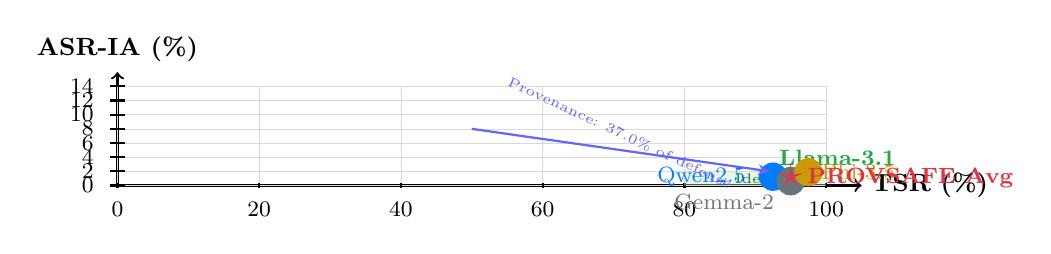
\begin{tikzpicture}[scale=0.09]
  % Axes
  \draw[thick, ->] (0,0) -- (105,0) node[right, font=\small\bfseries] {TSR (\%)};
  \draw[thick, ->] (0,0) -- (0,16) node[above, font=\small\bfseries] {ASR-IA (\%)};
  
  % Grid
  \draw[gray!30, very thin] (0,0) grid[xstep=20, ystep=2] (100,14);
  
  % Axis labels
  \foreach \x in {0,20,40,60,80,100} {
    \draw[thick] (\x,-0.3) -- (\x,0.3);
    \node[below, font=\footnotesize] at (\x,-1) {\x};
  }
  \foreach \y in {0,2,4,6,8,10,12,14} {
    \draw[thick] (-1,\y) -- (1,\y);
    \node[left, font=\footnotesize] at (-2,\y) {\y};
  }
  
  % Ideal region (high TSR, low ASR)
  \fill[lightgreen, opacity=0.4] (80,0) rectangle (100,2);
  \node[font=\tiny, success!70!black] at (90,1) {Ideal};
  
  % Data points
  % Llama-3.1-8B: TSR=95.0%, ASR=0.62%
  \fill[success] (95.0, 0.62) circle (2);
  \node[above right, font=\footnotesize\bfseries, success] at (92, 1.5) {\textbf{Llama-3.1}};
  
  % Qwen2.5-7B: TSR=92.5%, ASR=1.25%
  \fill[modelcolor] (92.5, 1.25) circle (2);
  \node[left, font=\footnotesize, modelcolor] at (90, 1.25) {Qwen2.5};
  
  % Gemma-2-9B: TSR=95.0%, ASR=0.62%
  \fill[secondary] (95.0, 0.62) circle (2);
  \node[below left, font=\footnotesize, secondary] at (94, 0.1) {Gemma-2};
  
  % Phi-3.5-Mini: TSR=97.5%, ASR=1.88%
  \fill[warning!80!black] (97.5, 1.88) circle (2);
  \node[right, font=\footnotesize, warning!80!black] at (98, 1.88) {Phi-3.5};
  
  % PROVSAFE Average: TSR=95.00%, ASR=1.09%
  \node[danger, font=\LARGE] at (95.00, 1.09) {$\star$};
  \node[right, font=\footnotesize\bfseries, danger] at (96, 1.09) {PROVSAFE Avg};
  
  % Arrow showing provenance contribution
  \draw[thick, ->, >=stealth, blue!60] (50, 8) -- (92, 2.0);
  \node[font=\tiny, blue!60, above, rotate=-25] at (70, 5.5) {Provenance: 37.0\% of defense};
  
\end{tikzpicture}
\end{document}
